\section{BCFW on-shell recursion}\label{sect-bcfw}
Tree-level amplitudes can be computed in using the singularities which appear when a propagator is put on-shell. 
Due to Britto, Cachazo, Feng and Witten~\cite{BRITTO2005499, PhysRevLett.94.181602}, one can establish a recursion relation for tree-level amplitudes by complex analysis (Cauchy's theorem).
The main idea is to take the external momenta to be complex and apply well chosen shifts to them.
This method does not require the knowledge of individual contribution of each diagram.
Let us see how this works in following~\cite{Elvang:2013cua}.
\\\\
Consider a tree-level n-point amplitude $A_n$ with massless external momenta.
The momenta of the external particles are $p_i$ for $i=1, \ldots, n$ with $p^2_i = 0$. 
The momentum conservation implies $\sum_{i=1}^n p_i^\mu = 0$. 
\\
Now, introduce $n$ complex vectors $r^{\mu}_i$ such that
\begin{enumerate}
\item $\sum_{i=1}^n r_i^{\mu}  = 0$
\item $r_i\cdot r_j = 0 \quad,\quad\forall i,j$
\item $p_i \cdot r_i = 0 \quad,\quad \forall i$
\end{enumerate}
We define the shifted momenta
\begin{equation*}
\hat{p}^\mu_i = p_i^{\mu} + z r_i^{\mu} \quad\textrm{with}\quad z\in\mathbb{C}
\end{equation*} 
It is easy to check that the momentum conservation holds for the shifted momenta and that the shifted momenta are themselves also null vectors.
We denote by $\hat{A}_n(z)$ the $n$-point amplitude computed in replacing the external momenta $p_i$'s in $A_n$ by the shifted ones. 
Note that $\hat{A}_n(z)$ is holomorphic and contains only simple poles $z_I$ in $z$\footnote{As one can see from a simple drawing, double or higher poles can not exist since they come from the propagators contained in an amplitude.}.
Then, by Cauchy's theorem, the unshifted amplitude $A_n = \hat{A}_n(z=0)$ is related to the shifted one by
\begin{equation}\label{residue}
A_n = - \sum_{z = z_I}\res\frac{\hat{A}_n(z)}{z} + B_n
\end{equation} 
where $B_n$ is the residue of the pole at $z = \infty$.
\\
There are some particular choices of shift such that $B_n = 0$.
Under these shifts, it suffices to compute only the first term of the above equation. 
Singularities appear when propagators are put on-shell. 
In the terms of the shifted momenta, they correspond to the poles of $\hat{A}(z)$.
Therefore, at tree-level, the poles of $\hat{A}(z)$ are the points where, for a non-trivial subset of generic momenta $\{p_i\}_{i\in I}$, 
\begin{equation*}
\hat{P}_I^2 := \big( \sum_{i\in I} \hat{p}_i \big)^2 = 0
\end{equation*}   
%
Then, one can check that
\begin{equation}\label{cauchy}
\res_{z=z_I}\frac{\hat{A}_n(z)}{z} = - \hat{A}_L(z_I)\frac{1}{P_I^2}\hat{A}_R(z_I)
\end{equation}
where 
\begin{equation*}
P_I := \sum_{i\in I}p_i
\end{equation*}
and $\hat{A}_{L,R}$ are two on-shell amplitudes with less external momenta connected by the on-shell propagator at two different ends (cf. figure~\ref{fig_cauchy}).
\begin{figure}[h]
  \centering
  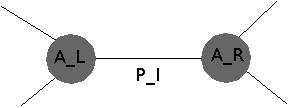
\includegraphics[width=0.5\linewidth]{bcfw.jpg}
  \caption{Illustration of~\cref{cauchy}. The two tree-level graphs $\hat{A}_{L,R}$ are on the two ends of a chosen combined momentun $P_I$}
  \label{fig_cauchy}
\end{figure}
\\
The BCFW recursion consists in applying a $[i,j\rangle$-shift :
\begin{equation}
|\hat{i}] = |i] + z |j], \quad |\hat{j}] = |j], \quad|\hat{i}\rangle = |i\rangle, \quad |\hat{j}\rangle = |j\rangle - z|i\rangle
\end{equation}  
with the rest of spinors remaining the same, 
and using the holomorphic property that we just reviewed.
\\
The term $B_n$ in~\cref{residue} will disappear when the shift is apply to ajacent lines $i,j$ for the following helicities~\cite{ArkaniHamed:2008yf}
\begin{equation*}
[-,-\rangle \quad [-,+\rangle \quad [+,+\rangle
\end{equation*}
Therefore, the unshifted amplitude can be computed by dropping the residue at infinity in~\cref{residue} and its first term on the right-hand side is given by~\cref{cauchy} under the BCFW shift.
%
\subsection{Example: $A_6[1^-2^-3^-4^+5^+6^+]$}
Let us now see how the BCFW recursion can be applied by considering a six-point next-to-MHV (NMHV) all-gluon amplitude $A_6[1^-2^-3^-4^+5^+6^+]$.
We assume that all external momenta are not collinear to each other.
For this example, we apply a $[1,6\rangle$-shift:
\begin{equation*}
|\hat{1}] = |1] + z|6]
\quad,\quad
|\hat{6}] = |6]
\quad,\quad
|\hat{1}\rangle = |1\rangle
\quad,\quad
|\hat{6}\rangle = |6\rangle - z|1\rangle
\end{equation*}
As discussed before, the first non-vanishing tree-level amplitudes are the three-point ones. 
There are thus three possible configuration for the external momenta \wrt the location of the propagator which will be taken on-shell\footnote{One can check that, whenever the shifted momenta $\hat{p}_1$ and $\hat{p}_6$ are put on the same side \wrt the on-shell propagator, there is no pole created.} (cf. figure~\ref{fig_A6nmhv})
\begin{figure}[h]
  \centering
  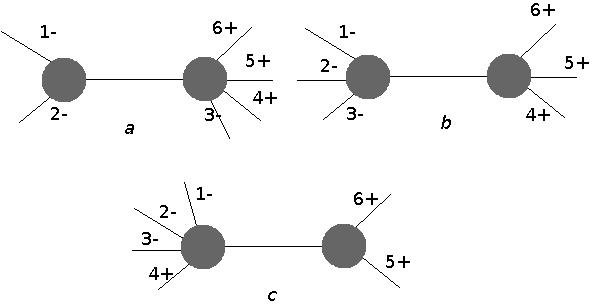
\includegraphics[width=0.8\linewidth]{A6nmhv.jpg}
  \caption{Possible contributions in the BCFW computation. The momenta $\hat{P}_I$ in the middle of each graphs are taken on-shell, \ie $\hat{P}_I^2=0$}
  \label{fig_A6nmhv}
\end{figure}
However, the configuration $b$ in~\ref{fig_A6nmhv} vanishes because it is impossible to find a helicity configuration for the intermediate momentum such that we have non-vanishing amplitudes on each side of it (the first non-vanishing four-point amplitudes are the MHV ones).
We are thus left with the configurations $a$ and $c$.
%
\paragraph{Configuration $a$}
To get a non-vanishing contribution on the left-hand ($\{1,2\}$) side of the on-shell propagator, we have to choose the propagator to have helicity plus at its left-hand end.
The contribution of this configuration is thus  
\begin{equation*}
\begin{split}
A_a = & \hat{A}_3[1^-,2^-, -P_{12}^+]\frac{1}{P_{12}^2}\hat{A}_5[3^-4^+5^+6^+ P_{12}^-]
\\
= &\frac{\langle \hat{1}2\rangle^3}{\langle 2\hat{P}_{12}\rangle\langle \hat{P}_{12} 1\rangle}
\frac{1}{[12]\langle 21\rangle}
\frac{\langle \hat{P}_{12} 3\rangle^4}{\langle 34\rangle\langle 45\rangle\langle 5\hat{6}\rangle\langle 6\hat{P}_{12}\rangle\langle \hat{P}_{12} 3\rangle}
\\
=&
\frac{\langle \hat{1}2\rangle^3}{\langle 2\hat{P}_{12}\rangle[\hat{P}_{12} 1][\hat{P}_{12} 1]\langle \hat{P}_{12} 1\rangle}
\frac{1}{[12]\langle 21\rangle}
\frac{\langle \hat{P}_{12} 3\rangle^3[\hat{P}_{12} 1]^3}{\langle 34\rangle\langle 45\rangle\langle 5\hat{6}\rangle\langle 6\hat{P}_{12}\rangle[\hat{P}_{12} 1]}
\end{split}
\end{equation*}
First, we determine the pole $z=z_I$ for this configuration by using the on-shell condition 
\begin{equation*}
\hat{P}_{12}^2 = 0
\quad\Rightarrow\quad
[\hat{1}2] =  [12] + z[62] = 0
\quad\Rightarrow\quad
z= -\frac{[12]}{[62]}
\end{equation*}
Also, we compute
\begin{equation*}
\begin{split}
& \langle 2 |\hat{\slashed{P}}_{12}|1] = z\langle 21\rangle[61] = -\frac{[12]}{[62]}\langle 21 \rangle[61]
\\
&
\langle 1 |\hat{\slashed{P}}_{12}|3\rangle = 
z[16]\langle 13 \rangle + [12]\langle 23 \rangle
=\frac{[21]}{[62]}\langle 3 |\slashed{P}_{12}|6]
\\
&
\langle \hat{6}\hat{P}_{12}\rangle[\hat{P}_{12}1] = z\langle 61 \rangle[61] + \langle 62\rangle - z\langle 12\rangle[21]
=
\frac{[12]}{[62]}P_{126}^2
\end{split}
\end{equation*}
Therefore
\begin{equation}\label{a6a}
A_a = -\frac{\langle 3 |\slashed{P}_{12}|6]^3}{[61]\langle 34\rangle \langle 45\rangle\langle 5|\slashed{P}_{16}|2]}[12]s_{126}
\end{equation}
%
%
\paragraph{Configuraion $c$}
This time, in order to get non-vanishing contribution, we impose the helicity of the intermediate propagator on the left-hand side to be minus.
\begin{equation*}
\begin{split}
A_c = & \hat{A}_5[1^-2^-3^-4^+ P_{56}^+]\frac{1}{P_{56}^2}\hat{A}_3[-P_{56},5^+,6^+]
\\
= &
\frac{[4\hat{P}_{56}]^4}{[4\hat{P}_{56}][\hat{P}_{56}\hat{1}][\hat{1}2][23][34]}\frac{1}{\langle 56\rangle [65]}\frac{[65]^3}{[5\hat{P}_{56}][\hat{P}_{56}6]}
\\
= &
\frac{[4\hat{P}_{56}]^3\langle\hat{P}_{56}1\rangle^3}{\langle 1P_{56}\rangle [\hat{P}_{56}\hat{1}][\hat{1}2][23][34]}\frac{1}{\langle 56\rangle [65]}\frac{[65]^3}{[5\hat{P}_{56}]\langle \hat{P}_{56} 1\rangle [\hat{P}_{56} 6]\langle 1\hat{P}_{56}\rangle}
\end{split}
\end{equation*}
The pole $z$ for this configuration is given by the on-shell condition, with the same computation as in the previous case
\begin{equation*}
\hat{P}_{56}^2 = 0 \quad\Rightarrow\quad
z=\frac{\langle 65\rangle}{\langle 15\rangle}
\end{equation*}
On the other hand
\begin{equation*}
\begin{split}
& \langle 1\hat{P}_{56}\rangle [\hat{P}_{56}\hat{1}] = \langle 15 \rangle[51] + \langle 16\rangle[61] + z\langle 15 \rangle[56] = P_{156}^2
\\
& [5\hat{P}_{56}]\langle\hat{P}_{56} 1 \rangle = [56]\langle 61\rangle
\\
&
\langle 1 \hat{P}_{56}\rangle[\hat{P}_{56}6] =\langle 15\rangle[56]
\end{split}
\end{equation*}
At the end, we get
\begin{equation}\label{a6c}
A_c = -\frac{[4|\slashed{P}_{56}|1\rangle^3}{s_{156}\langle 5|\slashed{P}_{16}|2][23][34]\langle 56\rangle\langle 61\rangle}
\end{equation}
To sum up, the total amplitude is
\begin{equation*}
A_6[1^-2^-3^-4^+5^+6^+] = A_a + A_c
\end{equation*}
where $A_a$ and $A_c$ are given in~\cref{a6a} and~\cref{a6c}.
